\let\negmedspace\undefined
\let\negthickspace\undefined
\documentclass[journal]{IEEEtran}
\usepackage[a5paper, margin=10mm, onecolumn]{geometry}
%\usepackage{lmodern} % Ensure lmodern is loaded for pdflatex
\usepackage{tfrupee} % Include tfrupee package

\setlength{\headheight}{1cm} % Set the height of the header box
\setlength{\headsep}{0mm}     % Set the distance between the header box and the top of the text
\usepackage{gvv-book}
\usepackage{gvv}
\usepackage{cite}
\usepackage{amsmath,amssymb,amsfonts,amsthm}
\usepackage{algorithmic}
\usepackage{graphicx}
\usepackage{textcomp}
\usepackage{xcolor}
\usepackage{txfonts}
\usepackage{listings}
\usepackage{enumitem}
\usepackage{mathtools}
\usepackage{gensymb}
\usepackage{comment}
\usepackage[breaklinks=true]{hyperref}
\usepackage{tkz-euclide} 
\usepackage{listings}
% \usepackage{gvv}                                        
\def\inputGnumericTable{}                                 
\usepackage[latin1]{inputenc}                                
\usepackage{color}                                            
\usepackage{array}                                            
\usepackage{longtable}                                       
\usepackage{calc}                                             
\usepackage{multirow}                                         
\usepackage{hhline}                                           
\usepackage{ifthen}                                           
\usepackage{lscape}
\begin{document}

\bibliographystyle{IEEEtran}
\vspace{3cm}

\title{1.11.12}
\author{EE24BTECH11030 - J.KEDARANANDA}
% \maketitle
% \newpage
% \bigskip
{\let\newpage\relax\maketitle}

\renewcommand{\thefigure}{\theenumi}
\renewcommand{\thetable}{\theenumi}
\setlength{\intextsep}{10pt} % Space between text and floats


\numberwithin{equation}{enumi}
\numberwithin{figure}{enumi}
\renewcommand{\thetable}{\theenumi}


\textbf{Question}:\\
If the sum of 2 vectors is a unit vector , prove that the magnitude of their difference is $\sqrt{3}$.\hfill{\brak{12,2018}}\\
\\ \solution \\
    \begin{table}[h!]    
      \centering
      \begin{center}
    \begin{tabular}{|c|c|} 
        \hline
            \textbf{Variable} & \textbf{Value} \\ 
        \hline
            $\boldsymbol{BC}$ & 6 cm \\ 
        \hline
            $\boldsymbol{AB}$ & 5 cm \\ 
        \hline
            $\angle \vec{B}$  & $60^\circ$ \\
        \hline
    \end{tabular}
\end{center}  



      \caption{}
    \end{table}
    \begin{align}
        \abs{\abs{\vec{A}}} = \abs{\abs{\vec{B}}} = 1 \\ \label{eq1.11.12.1}
        \abs{\abs{\vec{A}+\vec{B}}} = 1 
    \end{align}
    \begin{align}
        \abs{\abs{\vec{A}+\vec{B}}}^2 = \abs{\abs{\vec{A}}}^2 + \abs{\abs{\vec{B}}}^2 + 2\brak{\vec{A} \cdot \vec{B}}\label{eq1.11.12.2}
    \end{align}
    \begin{align}
        1 = 2 + 2\brak{\vec{A} \cdot \vec{B}} \label{eq1.11.12.3}
    \end{align}
    \begin{align}
        \brak{\vec{A} \cdot \vec{B}} = \frac{-1}{2} \label{eq1.11.12.4}
    \end{align}
    \begin{align}
        \abs{\abs{\vec{A}-\vec{B}}}^2 = \abs{\abs{\vec{A}}}^2 + \abs{\abs{\vec{B}}}^2 - 2\brak{\vec{A} \cdot \vec{B}} \label{1.11.12.5}
    \end{align}
    \begin{align}
        \abs{\abs{\vec{A}-\vec{B}}}^2 = 1 + 1 + 1 \label{1.11.12.6} 
    \end{align}
    \begin{align}
        \abs{\abs{\vec{A}-\vec{B}}}^2 = 3 \\
        \abs{\abs{\vec{A}-\vec{B}}} = \sqrt{3}
    \end{align}
    \begin{figure}[h]
        \centering
       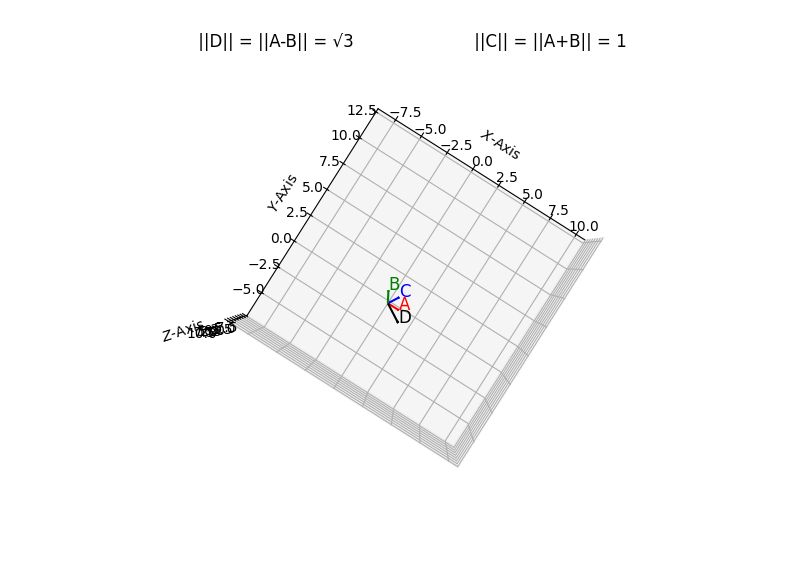
\includegraphics[width=\linewidth]{figs/fig1.png}
       \caption{}
       \label{graph}
    \end{figure}



\end{document}  







